\chapter{From listings to an application}
\label{chap:body}

This chapter follows the project from raw listings to a deployed tool: the data, the selection of a model under rules fixed in advance, its single evaluation on held-out listings, and the application built on it.

\section{Data collection and cleaning}

On 17 September 2026 a purpose-built crawler collected 2,178 for-sale iPhone listings from Tori. It fetched only paths allowed by \texttt{robots.txt} and sent at most one request every three seconds. Data were minimised at collection time: seller identifiers, coordinates, postal codes and photos were never stored, and contact details were scrubbed from titles and descriptions. An audit found eleven contact details the first scrubber had missed, so we extended it and re-scrubbed the data; because descriptions may still name people, the repository is private. The canvas planned to use Tori only with written permission and the eBay Browse API otherwise; collection instead proceeded with the course supervisor's approval, a deviation we record here.

Cleaning removed accessories, spare parts, placeholder prices, multi-phone bundles and one Samsung phone, leaving 2,007 listings. We derived the exact model (51 models from 2008 to 2026), release year, storage (96\% of listings), battery health (51\%) and negation-aware text flags such as mentioned damage. Reposts of the same advertisement were grouped by their text, and 20\% of the listings (405), grouped in the same way, were held out as a test set used only once. On the 1,602 development listings, asking prices were right-skewed (skewness 1.57, against $-0.46$ for log prices). Relative to the median price of the same model and storage, retailers asked about 22\% more, phones needing repair about 60\% less and listings mentioning damage about 22\% less.

\section{Model selection}

Because effects such as these are multiplicative, all models were trained on $\log(1+\text{price})$ and compared by the root mean squared logarithmic error (RMSLE); we also report the mean absolute error (MAE). Every score came from the same five-fold grouped cross-validation, with all preprocessing inside scikit-learn pipelines on training folds only \parencite{pedregosa2011scikit}. Inputs were limited to what a user knows before posting an advertisement. A feature check kept the phone model, condition, storage, seller type and mentioned damage, and dropped battery, region and the other text flags, which changed the RMSLE by 0.002 or less. Five tuned model families were compared with a lookup baseline, the median price of the same model and storage (Table~\ref{table:cv}).

\tagpdfsetup{table/header-rows={1}}
\begin{table}[ht!]
\centering
\begin{tabular}{l c c}
\toprule
Model & RMSLE & MAE (euros) \\
\midrule
Lookup baseline & $0.369 \pm 0.022$ & $56 \pm 4$ \\
Linear regression & $0.312 \pm 0.031$ & $53 \pm 3$ \\
Decision tree & $0.308 \pm 0.017$ & $51 \pm 3$ \\
Random forest & $0.293 \pm 0.016$ & $49 \pm 5$ \\
Support vector regression & $0.292 \pm 0.016$ & $47 \pm 4$ \\
Gradient boosting & $0.284 \pm 0.015$ & $47 \pm 3$ \\
\bottomrule
\end{tabular}
\caption{Cross-validated scores on the 1,602 development listings (mean $\pm$ standard deviation over five grouped folds).}
\label{table:cv}
\end{table}

Gradient boosting \parencite{friedman2001greedy}, with 400 rounds of four-leaf trees, had the lowest RMSLE and was the only model within one standard error, the rule set in advance. Its grid was widened three times, giving it more tuning than the others, and two models were within about 0.01, so the choice is close.

\section{Held-out results and price ranges}

Scored once on the 405 test listings, the model's RMSLE was 27\% below the baseline's (95\% CI 19--35\%), with confidence intervals from 2,000 bootstrap resamples by advertisement group (Table~\ref{table:test}; \cite{efron1993introduction}). All success criteria set before modelling were met.

\tagpdfsetup{table/header-rows={1}}
\begin{table}[ht!]
\centering
\begin{tabular}{l c c}
\toprule
Metric & Final model & Lookup baseline \\
\midrule
RMSLE & 0.272 (0.242--0.302) & 0.374 (0.331--0.418) \\
MAE (euros) & 46 (42--52) & 58 (51--64) \\
Median percentage error & 14.3\% & 16.5\% \\
80\% range coverage & 77\% & -- \\
\bottomrule
\end{tabular}
\caption{Results on the 405 held-out test listings, with 95\% bootstrap confidence intervals.}
\label{table:test}
\end{table}

Because one number hides uncertainty, each estimate comes with an 80\% range: a conformal interval built from out-of-fold errors, with a separate width per launch period in the spirit of Mondrian conformal prediction \parencite{vovk2005algorithmic}. Old phones, which are harder to price, get wider ranges (a factor of 1.97 for 2016 or earlier against 1.19 for 2023 or later). The ranges covered 77\% of test listings, 78\% for private sellers and 75\% for retailers. Errors were uneven, with a median of 7\% for phones from 2023 or later but 27\% for 2016 or earlier; the weakest group was the 82 listings asking under 100~euros, often broken phones listed as working, where estimates were 28\% too high on average and the ranges covered only 65\%.

\section{The application}

After the test, the model was retrained on all 2,007 listings and served by a Flask application at \url{https://priced-right.onrender.com} that offers both modes (Figure~\ref{fig:app}). It validates every input on the server, draws the range as a bar, flags rough estimates and stores nothing a user enters.

\begin{figure}[ht!]
\centering
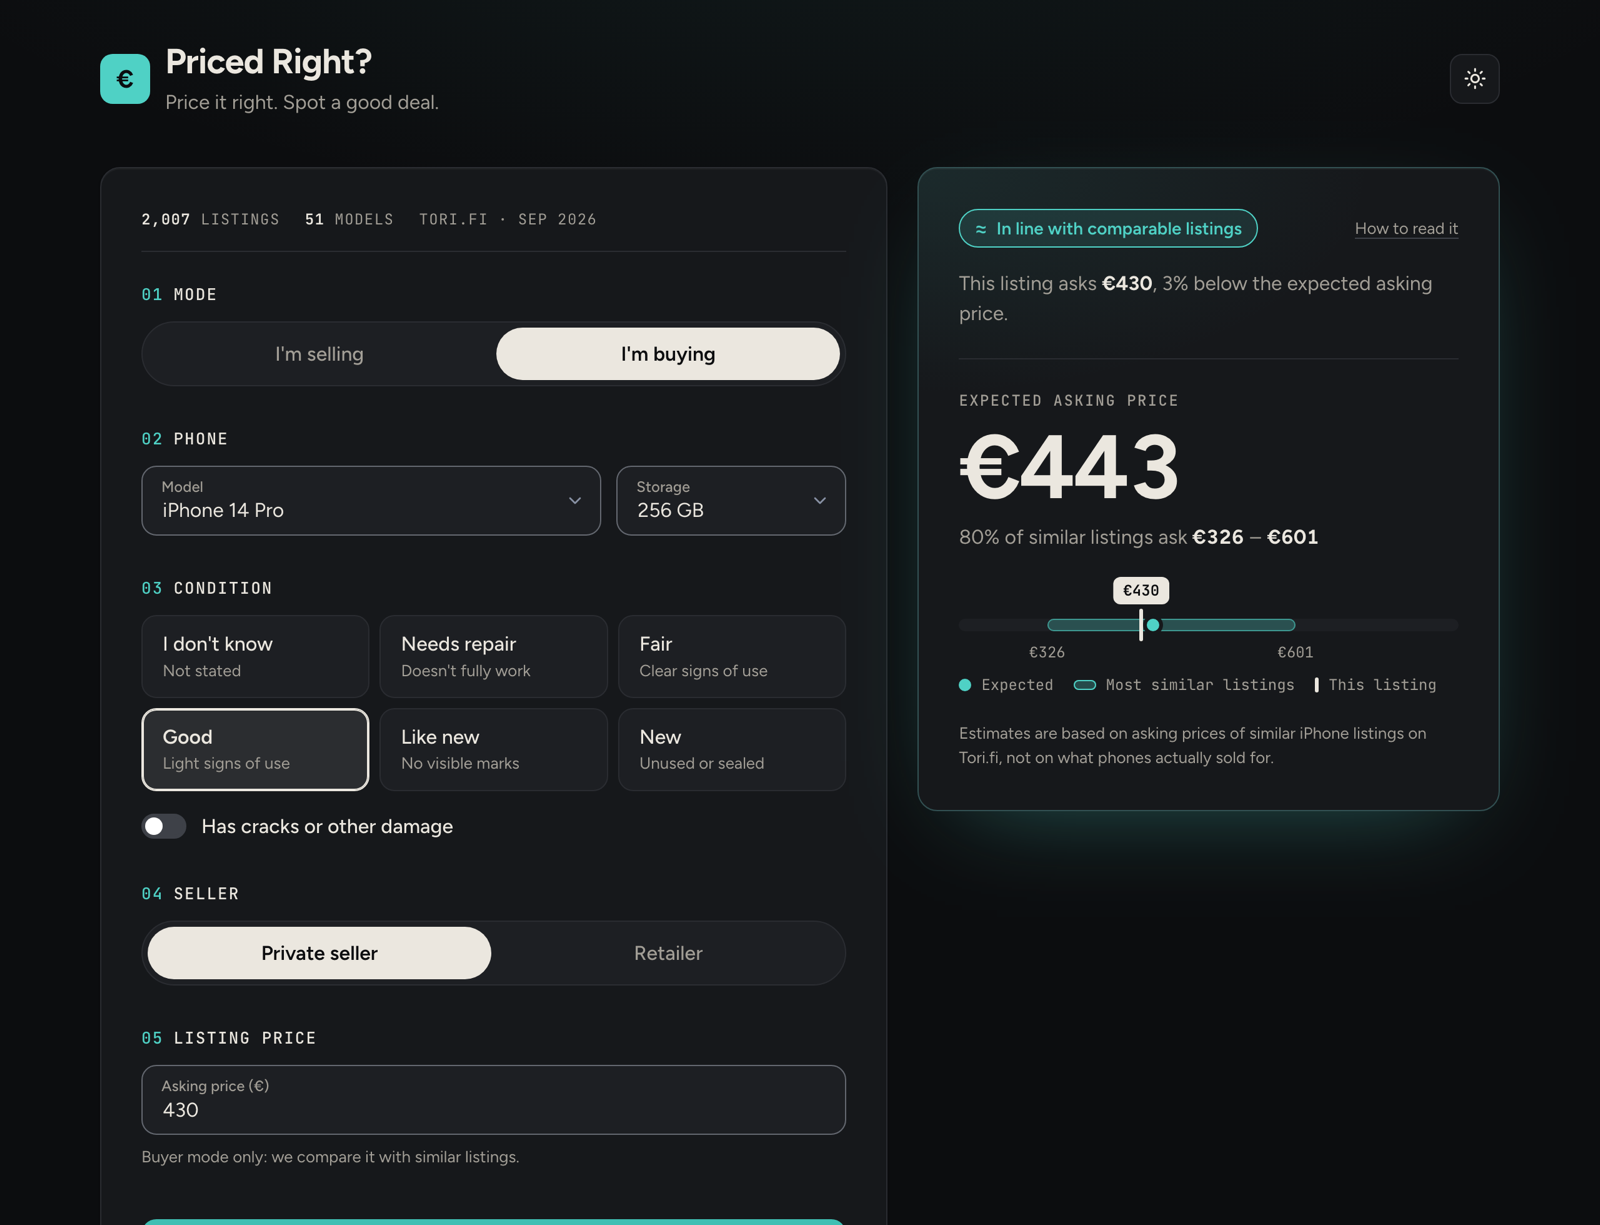
\includegraphics[alt={Screenshot of the Priced Right application in buyer mode. The form on the left has an iPhone 14 Pro, 256 GB, good condition and a listing price of 430 euros. The result card on the right says In line with comparable listings, shows an expected asking price of 443 euros, a range of 326 to 601 euros, and a bar with the listing marked inside the range.}, width=0.46\textwidth]{figures/app.png}
\caption{The application in buyer mode: a listing at 430~euros is in line with comparable listings.}
\label{fig:app}
\end{figure}
